\chapter{基于多分区的自适应均衡技术}

如第二章所述，本文提出的多分区回读模型已为不同区域生成了具有区分度的信道响应特征。本章以此为基础，致力于设计一种


\section{自适应均衡技术架构}

\subsection{问题分析}

\subsection{技术架构}

本章提出的多通道自适应均衡系统架构如图\ref{fig:ch.cnn2.sys}所示。该架构在经典部分响应最大似然（PRML）检测框架基础上，针对高密度AD光盘信道中码间干扰（ISI）与轨道间串扰（ITI）的多维耦合特性进行了关键性改进。系统采用多通道并行处理架构，通过数字均衡器、自适应均衡器、检测模块及LMS更新模块的协同工作，实现对读出信号的精确均衡与恢复。系统输入为来自第三章所述多分区建模生成的多个通道的原始读出信号（包括主轨道及相邻轨道信号），输出为经均衡与检测恢复出的二进制数据序列。

\begin{figure}[h]
	\centering
	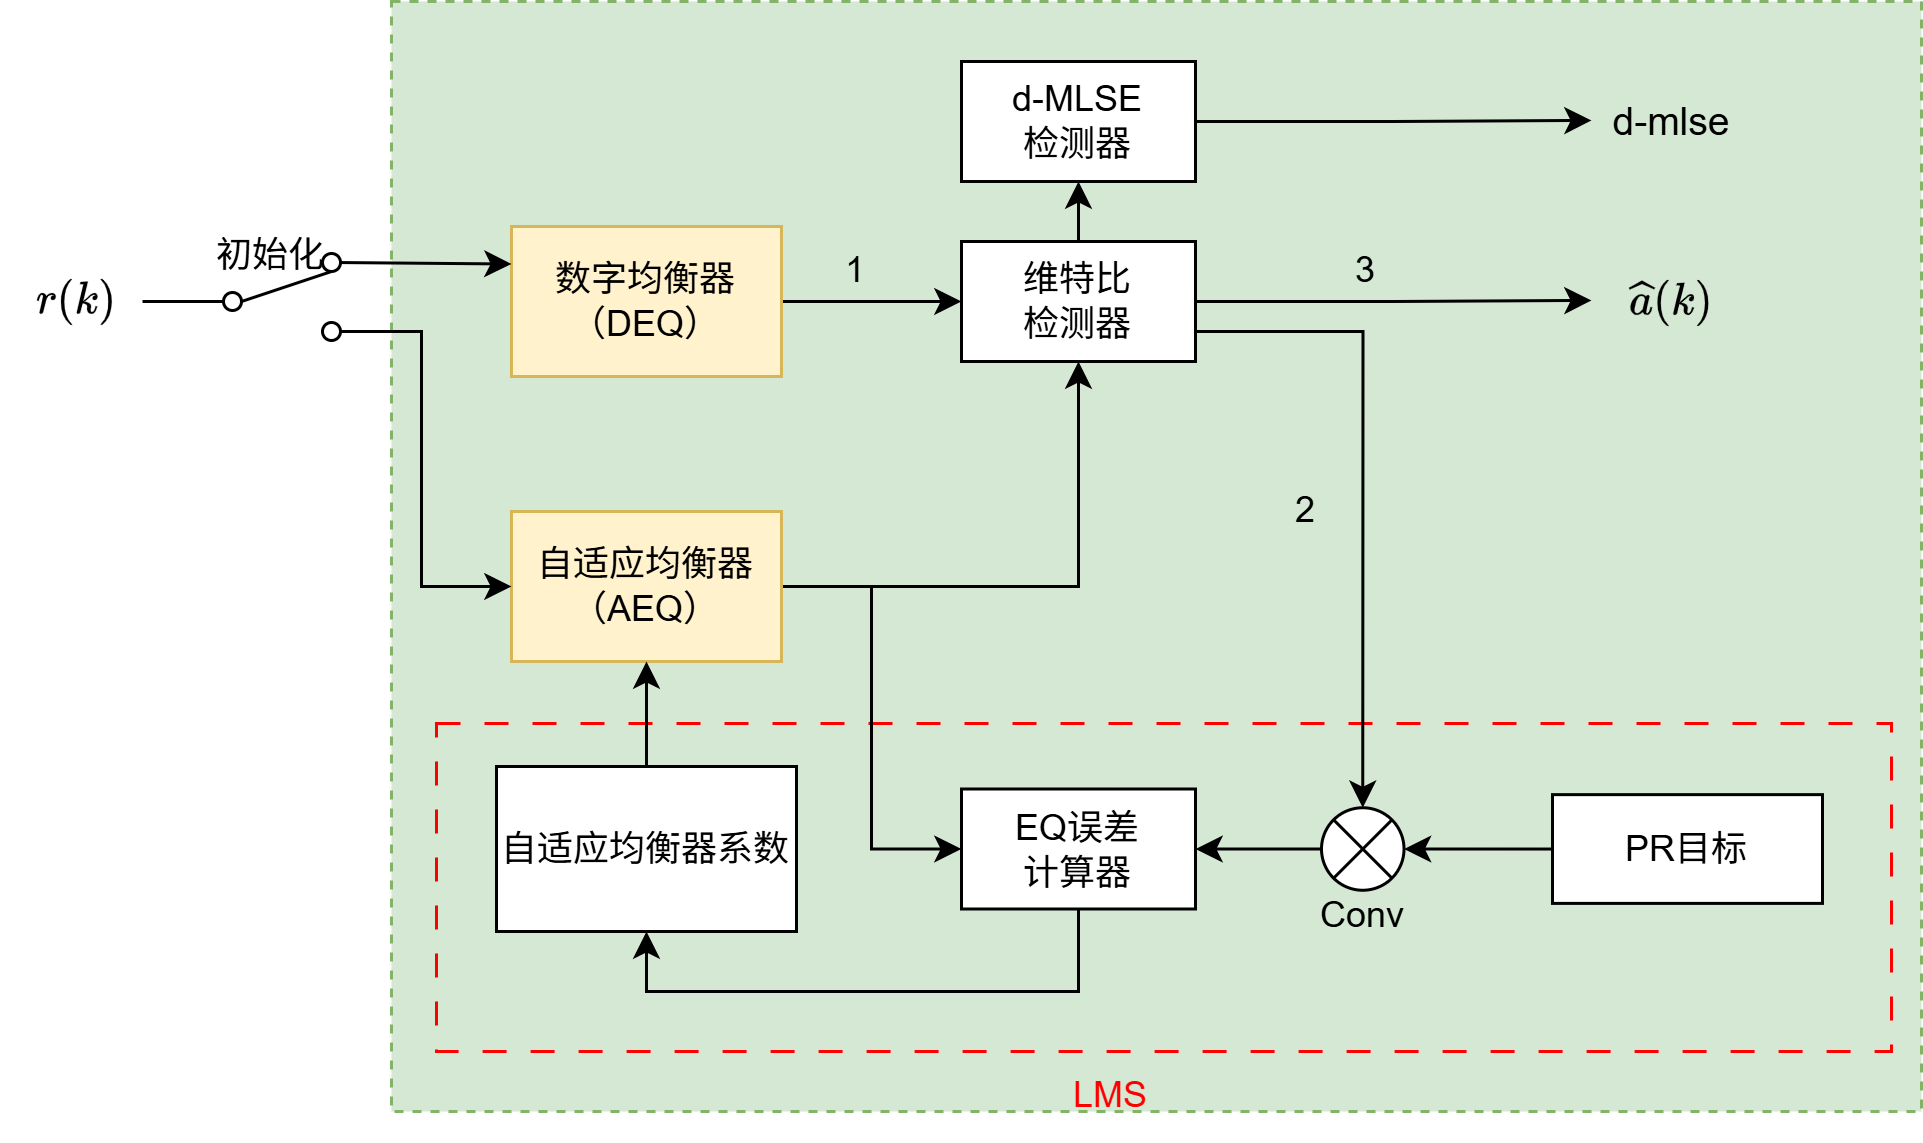
\includegraphics[width=0.9\textwidth]{float/ch.cnn2/SYS.png}
	\caption{基于PRML的多通道自适应均衡系统总体架构图\label{fig:ch.cnn2.sys}}
\end{figure}

各核心功能单元分述如下：

\textbf{1. 数字均衡器}

数字均衡器是系统的首次运行时的前级信号处理单元，主要负责对原始多通道输入信号进行初步整形与线性补偿，为后续的自适应均衡提供一个良好的初始化信号条件。该模块采用固定的滤波器结构，其系数依据信道特性预先设定。

\textbf{2. 自适应均衡器}

自适应均衡器是本系统的核心处理单元，位于数字均衡器之后。它通过可动态调整的滤波器系数，实时跟踪信道的变化并抑制包括ISI和ITI在内的复杂干扰。每个通道拥有独立的自适应均衡器，其输出经融合后形成最终的均衡信号。

\textbf{3. LMS更新模块}

LMS更新模块是实现系统自适应能力的关键闭环控制单元。该模块首先根据检测模块的输出与预设的部分响应（PR）目标，生成理想的参考信号；然后计算该参考信号与实际均衡输出之间的误差；最后，利用该误差信号，通过LMS算法驱动自适应均衡器的系数进行迭代更新，从而持续优化系统的均衡性能。

\textbf{4. 检测模块}

检测模块负责从均衡后的信号中恢复出原始数据序列。它主要由两部分构成：一部分是基于延迟判决的d-MLSE单元，为最终信号质量评估提供参考；另一部分是经典的维特比检测器，负责执行最大似然序列估计，输出最终的解码比特流。

通过上述四个核心模块的协同与闭环运作，整个系统能够动态适应高密度AD光盘信道的复杂特性，有效抑制多维干扰，为数据的可靠恢复提供保障。


\textbf{1. 首次信号处理（初始化阶段）}
首次处理的主要目标是建立初始的均衡器系数，为系统提供一个稳定的自适应起点。其具体流程如下：
\begin{enumerate}
	\item \textbf{预设均衡处理}：来自多个分区的原始信号首先通过一个系数预先设定的数字均衡器。该处理对信号进行初步的线性整形，补偿信道的主要频率失真，为后续检测提供相对规整的波形。
	\item \textbf{初始检测与目标信号生成}：经数字均衡器处理后的信号被送入维特比检测器，进行首次数据恢复。检测器输出的初步比特判决序列，与预设的部分响应（PR）目标多项式进行卷积运算，生成一个理想的“目标信号”。该目标信号代表在理想信道条件下，当前数据序列应有的标准波形。
	\item \textbf{误差计算与系数训练}：计算数字均衡器输出信号与目标信号之间的差异，得到初始的均衡误差。算法根据误差大小和方向，基于数字均衡器的初始值迭代计算出能够显著减小该误差的一组优化滤波器系数。这组系数将被设定为自适应均衡器的初始工作参数。
	\item \textbf{自适应均衡与最终评估}：随后，同一批首次信号将再次被处理，但此次改为通过已更新系数的自适应均衡器。经过更精细的自适应均衡后，信号再次进入检测环路。维特比检测器进行最终判决，输出二进制数据序列。同时，d-MLSE 单元利用这一判决，对本次处理的信号质量进行评估，并输出相应的度量结果（如d-mlse值），作为系统性能的初始参考。
\end{enumerate}

\textbf{2. 后续信号处理（连续工作阶段）}
在完成首次信号的初始化训练后，系统进入高效的连续工作模式。后续到来的数据流将直接利用已训练好的自适应均衡器进行处理，流程大大简化：
\begin{enumerate}
	\item \textbf{直接自适应均衡}：后续的输入信号跳过预设的数字均衡器，直接进入已经具有优化系数的自适应均衡器进行均衡处理。
	\item \textbf{闭环检测与更新}：均衡后的信号立即进入由维特比检测器、PR目标卷积、误差计算和LMS更新构成的闭环。在此闭环中，检测结果被用于实时生成目标信号并计算误差，该误差随即驱动LMS算法对自适应均衡器的系数进行微调，使之能够跟踪信道的缓慢变化或抵抗突发干扰。
	\item \textbf{实时输出}：维特比检测器持续输出恢复的二进制数据流，同时d-MLSE单元提供实时的信号质量评估输出。
\end{enumerate}

本系统通过上述流程设计，实现了三大核心功能：
\begin{itemize}
	\item \textbf{快速初始化}：利用首次信号完成自适应均衡器系数的快速、有效训练，避免了传统自适应均衡器因初始系数不当导致的收敛慢或不收敛问题。
	\item \textbf{持续自适应}：在连续工作阶段，系统构成一个实时闭环，能够动态跟踪信道特性的变化，并对均衡器系数进行在线微调，保持优异的干扰抑制能力。
	\item \textbf{高质量恢复与监控}：最终，系统不仅稳定输出低误码率的二进制数据，还通过d-MLSE单元提供实时的内在性能评估，为系统状态监控和后续的PR目标动态优化提供了关键信息。
\end{itemize}

此流程设计确保了系统从启动到稳定工作的平滑过渡，兼顾了初始化阶段的鲁棒性与工作阶段的高效性，为高密度AD光盘的可靠数据读取提供了坚实的处理框架。

\section{基于LMS的多通道自适应均衡方法}

\subsection{多通道数字均衡器}

多通道数字均衡器是系统初始化阶段的关键预处理模块，其核心功能在于对来自多个分区的原始回读信号进行初步的线性整形与频率补偿。通过对原始信号中由信道非理想特性引入的主要频率失真进行校正，该模块能够将输入波形初步规整至接近预设部分响应（PR）目标形状，从而为后续的自适应均衡处理提供一个相对稳定、干扰得到初步抑制的输入信号环境。这一预处理步骤对于保障整个自适应均衡系统能够快速、平稳地收敛至最优工作状态具有至关重要的作用。

本设计采用基于并行多通道架构的有限冲激响应（FIR）滤波器结构实现数字均衡器。该架构与第三章所述的多分区回读模型（例如，图\ref{fig:ch.cnn1.Pattern_P1}中所示的六分区模式）紧密对应，确保来自不同空间分区（如主轨道及其相邻轨道）的读出信号能够经由各自独立的FIR滤波器通路进行处理。这种并行化的设计使得系统能够根据各分区信道的具体特性差异，实施初步的、有针对性的线性补偿，为后续更精细的自适应处理奠定基础。

数字均衡器的性能在很大程度上取决于其滤波器系数 $\mathbf{w}_{\text{DEQ}, m}$ 的准确性。与运行过程中动态调整系数的自适应均衡器不同，数字均衡器的系数是在系统初始化阶段通过一次性的离线训练过程预先计算确定的。该训练过程利用仿真生成的高信噪比理想信道回读信号作为训练序列，旨在获得一组能够有效补偿信道确定性失真的固定滤波器系数。具体而言，系数的设计过程可概括为两个递进的阶段。首先，基于最小均方（LMS）算法的系数粗调阶段。在此阶段，以一个结构相同的临时滤波器模型，利用无噪声的理想回读信号及其对应的理想PR目标信号作为期望响应，采用LMS算法进行迭代训练。LMS算法通过最小化滤波器实际输出与期望信号之间的瞬时误差平方，逐步调整滤波器权值向量 $\mathbf{w}$，其更新遵循
\begin{align}
 	\mathbf{w}(n+1) = \mathbf{w}(n) + \mu \cdot e(n) \cdot \mathbf{x}(n)
\end{align}
 的规则，其中 $e(n)$ 为误差，$\mu$ 为固定步长，$\mathbf{x}(n)$ 为输入向量。该阶段能够快速获得一组逼近信道主要线性失真特性的基础系数。随后，进入基于变步长归一化最小均方（VSNLMS）算法的系数微调阶段。VSNLMS算法在NLMS算法的基础上引入自适应步长机制，其更新公式为 
 \begin{align}
 \mathbf{w}(n+1) = \mathbf{w}(n) + \frac{\mu(n)}{\|\mathbf{x}(n)\|^2 + \delta} \cdot e(n) \cdot \mathbf{x}(n)
\end{align}
 其中，时变步长 $\mu(n)$ 可根据误差信号 $e(n)$ 动态调节，以在收敛速度与稳态失调之间取得平衡；归一化项使算法对输入信号幅度变化具有鲁棒性；小常数 $\delta$ 用于防止数值不稳定。此阶段的微调进一步提升了滤波器系数对实际环境中可能存在的轻微扰动（如信号幅度波动）的适应性，增强了均衡器的整体鲁棒性。

在完成上述系数训练后，为进一步优化性能，通常会对获得的系数进行扩展处理，例如在核心系数序列前后补零以增加滤波器长度。这种扩展操作在时域上相当于对滤波器的冲激响应施加了平滑窗函数，在频域上则使滤波器的频率响应曲线更为平缓。此举的目的主要有两方面：其一，为后续的自适应均衡器提供一个更为宽松的优化起始点和平滑的误差曲面，有助于其更快、更稳定地收敛；其二，更长的滤波器长度通常意味着更强的带外噪声抑制能力，有助于提升系统在低信噪比环境下的表现。

从信号处理的角度进行形式化描述，假设系统包含 $M$ 个独立通道，第 $m$ 个通道在离散时间索引 $k$ 的输入信号为 $r_{m,k}$。经过离线训练与扩展后，该通道的数字均衡器由一组长度为 $N_{\text{DEQ}}$ 的固定抽头系数 $\{w_{\text{DEQ}, m, i}\}_{i=0}^{N_{\text{DEQ}}-1}$ 定义，其输出信号 $y_{m,k}$ 通过离散线性卷积计算得出：
\[
y_{m,k} = \sum_{i=0}^{N_{\text{DEQ}}-1} w_{\text{DEQ}, m, i} \cdot r_{m, k-i}
\]
整体而言，多通道数字均衡器模块可被视为一个多输入多输出（MIMO）的线性时不变系统。该系统接收来自各分区的原始信号向量 $\mathbf{r}_k = [r_{1,k}, r_{2,k}, \ldots, r_{M,k}]^T$ 作为输入，并产生经过初步均衡处理后的输出信号向量 $\mathbf{y}_k = [y_{1,k}, y_{2,k}, \ldots, y_{M,k}]^T$。其全局输入输出关系可简洁地表述为：
\[
\mathbf{y}_k = \mathbf{W}_{\text{DEQ}} * \mathbf{r}_k
\]
其中，$\mathbf{W}_{\text{DEQ}}$ 是一个维度为 $M \times N_{\text{DEQ}}$ 的滤波器系数矩阵，汇集了所有通道的固定系数；符号 `*` 在此表示按通道独立进行的卷积运算。该模块通过上述设计，为整个自适应均衡系统提供了至关重要的信号预处理功能。

\subsection{多通道自适应均衡器}

自适应均衡器模块位于数字均衡器之后，是本系统实现动态干扰抑制与最终PR目标精确匹配的核心功能单元。其主要任务在于实时跟踪信道特性的时变与非线性成分，并对前级数字均衡器未能完全消除的残余失真，特别是高密度记录条件下由衍射极限和轨道耦合效应引发的动态码间干扰（ISI）与轨道间串扰（ITI），进行精细化的补偿。

该模块同样采用有限冲激响应滤波器结构，但其根本特征在于滤波器系数能够依据实时反馈的误差信号进行动态更新，从而具备自适应能力。自适应均衡器的输入信号来源于前级数字均衡器处理后的多通道输出 $\mathbf{y}_k = [y_{1,k}, y_{2,k}, \ldots, y_{M,k}]^T$。对于第 $m$ 个通道，假设其自适应均衡器的长度为 $N_{\text{AEQ}}$，则在时刻 $k$，该通道的输出 $z_{m,k}$ 通过其时变系数 $\{w_{\text{AEQ}, m, j}(k)\}_{j=0}^{N_{\text{AEQ}}-1}$ 与输入信号 $\{y_{m, k-j}\}$ 的卷积计算获得：
\[
z_{m,k} = \sum_{j=0}^{N_{\text{AEQ}}-1} w_{\text{AEQ}, m, j}(k) \cdot y_{m, k-j}
\]
所有 $M$ 个通道的输出共同构成向量 $\mathbf{z}_k = [z_{1,k}, z_{2,k}, \ldots, z_{M,k}]^T$。为生成最终的、用于后续检测的均衡信号 $s_k$，本设计采用加权融合策略对各通道输出进行合成，即：
\[
s_k = \sum_{m=1}^{M} \alpha_m \cdot z_{m,k}
\]
式中，$\alpha_m$ 代表第 $m$ 个通道的融合权重。权重分配策略可以根据具体需求进行设计，例如，赋予携带主轨道信息通道较高权重，而根据辅助轨道对主轨道干扰的贡献度或相关性来设定其权重。更为先进的策略可使 $\alpha_m$ 基于实时的信号质量度量（如信噪比估计）进行自适应调整，以优化整体性能。

自适应均衡器系数的更新机制基于最小均方误差准则。该机制旨在通过迭代调整滤波器系数，最小化最终均衡信号 $s_k$ 与一个理想参考信号 $d_k$ 之间的均方误差。参考信号 $d_k$ 通常由检测环节提供：维特比检测器对均衡信号 $s_k$（或其延迟版本）进行硬判决，得到比特序列估计 $\hat{a}_k$，然后将该序列与预设的PR目标多项式进行卷积，从而重构出在理想信道条件下应有的信号波形 $d_k = \sum_{l} pr_l \cdot \hat{a}_{k-l}$。

标准的LMS算法通过瞬时误差 $e(k) = d_k - s_k$ 来驱动系数更新。对于第 $m$ 个通道，其系数向量 $\mathbf{w}_{\text{AEQ}, m}(k)$ 的更新遵循以下规则：
\[
\mathbf{w}_{\text{AEQ}, m}(k+1) = \mathbf{w}_{\text{AEQ}, m}(k) + \mu \cdot e(k) \cdot \mathbf{y}_{m, k}
\]
其中，$\mathbf{y}_{m, k} = [y_{m,k}, y_{m,k-1}, \ldots, y_{m,k-N_{\text{AEQ}}+1}]^T$ 是该通道在当前时刻的输入向量，$\mu$ 为控制算法收敛特性的步长参数。

考虑到硬件实现的复杂性与资源消耗，本设计在实际采用时使用了符号-误差LMS算法的一种简化形式。该算法仅利用误差信号 $e(k)$ 的极性（符号）信息来指导系数更新，其更新公式为：
\[
\mathbf{w}_{\text{AEQ}, m}(k+1) = \mathbf{w}_{\text{AEQ}, m}(k) + \mu \cdot \operatorname{sign}[e(k)] \cdot \mathbf{y}_{m, k}
\]
这里，符号函数定义为： 
\[
\operatorname{sign}(x) = 
\begin{cases} 
	1, & \text{if } x > 0 \\
	0, & \text{if } x = 0 \\
	-1, & \text{if } x < 0 
\end{cases}
\]
虽然这种简化在一定程度上可能影响算法的收敛速度，但它显著降低了每次更新所需的计算量（特别是乘法运算次数），使其更加适合于对功耗和计算资源有严格限制的实时处理系统或专用集成电路实现。

自适应均衡处理流程主要涵盖两个连续阶段。首先是卷积阶段，在此阶段，数字均衡器的多通道输出 $\mathbf{y}_k$ 分别与各自对应的、实时更新的自适应均衡器系数进行卷积运算，生成各通道的初步均衡结果 $z_{m,k}$。随后是融合与归一化阶段。在此阶段，首先按照预设的权重 $\alpha_m$ 将各通道的 $z_{m,k}$ 进行加权求和，得到一个融合后的信号。紧接着，对该融合信号实施归一化处理。归一化的核心目的在于使最终输出的均衡信号 $s_k$ 具有与理想参考信号 $d_k$ 相匹配的幅度动态范围。这一步骤对于确保后续检测器（如维特比检测器）能够在其设计的最优判决门限下稳定工作至关重要。归一化功能可以通过集成自动增益控制环路或应用简单的幅度缩放因子来实现。


\subsection{检测与信号质量评估}

检测与信号质量评估模块在系统链路中承担着最终数据恢复与内在性能评估的关键职责。该模块主要由维特比（Viterbi）检测器与基于分布的最大似然序列误差估计（d-MLSE）单元共同构成。其中，维特比检测器作为核心检测单元，通过对均衡后信号执行最大似然序列估计（MLSE），实现原始数据比特流的恢复；而d-MLSE单元则在不依赖实际误码统计的情况下，提供一种能够实时、定量反映信号检测可靠性的内在质量评估手段。

\subsubsection{基于状态优化的维特比检测器}

维特比算法作为一种基于动态规划的最大似然序列检测算法，其基本思想是通过在网格图（Trellis）上进行状态度量的递归计算与路径选择，寻找与接收序列匹配概率最高的发送序列。在本系统框架下，经均衡处理后的信号 $s_k$ 被输入至维特比检测器。假设系统采用的部分响应（PR）目标约束长度为 $L$，相应的信道记忆长度为 $L-1$，则理论网格图中每个时刻需处理的状态数目为 $2^{L-1}$。算法执行过程中，针对每一个可能的状态转移分支，需要计算其分支度量（Branch Metric）。该度量表征了实际观测信号 $y$（即 $s_k$ 的采样值）与在该分支假设下、根据PR目标及分支对应符号序列所重构的理想信号之间的欧氏距离平方，具体计算公式如下：

\[
bm_{j,i} = \left( y - \sum_{t=0}^{L-1} a_t \cdot d(j,i)_t \right)^2
\]

式中，$a_t$ 表示PR目标多项式的系数，$d(j,i)$ 代表从状态 $j$ 转移至状态 $i$ 所对应的长度为 $L$ 的符号序列。在此基础上，状态度量（State Metric）依据“累积代价最小”原则进行更新。对于当前时刻 $t$ 的某个状态 $i$，其状态度量 $sm_i(t)$ 通过比较所有可能前驱状态 $j$ 的累积度量与该状态转移分支度量之和的最小值来确定，即：

\[
sm_i(t) = \min_{j \in \text{前驱状态集合}} \{ sm_j(t-1) + bm_{j,i} \}
\]

随着信号序列的持续输入，算法逐步更新各状态度量并记录相应的幸存路径。待全部信号处理完毕后，选取具有最小终态度量的路径作为最大似然路径，并通过回溯操作输出对应的判决比特序列 $\hat{a}_k$。

随着记录密度的提升，为匹配信道特性可能需要采用更长的PR目标，这将导致网格图状态数目呈指数增长，进而显著增加检测器的计算复杂度和硬件资源消耗。为应对这一挑战，本设计对维特比检测器实施了两项关键性优化。首先，充分利用系统所采用的PCWA110游程限制（RLL）编码的约束特性。该编码为$(1,10)$ RLL码，其编码规则禁止连续出现`1`至`0`或`0`至`1`的跃迁。依据此约束，可在构建网格图时预先排除所有违反该规则的状态转移路径，从而大幅削减有效需处理的状态数量。如表\ref{tab:pruned_states}所示，经过此项剪枝优化后，即使在PR目标长度达到11的情况下，所需处理的状态数也由理论上的1024个锐减至178个，有效缓解了“状态爆炸”问题，提升了检测效率。其次，为规避传统维特比算法最终阶段耗时的路径回溯操作，本设计采用了一种基于路径存储器的免回溯输出策略。该方法为网格图中的每一个状态维护一个固定长度的路径记忆寄存器。在每次状态度量更新的同时，将选中前驱状态对应的幸存路径进行移位，并将当前分支所决定的比特值存入寄存器末端。当信号序列处理完成时，直接读取终态中具有最小状态度量所对应的路径寄存器内容，即可获得最终的检测结果。该策略以增加寄存器存储资源为代价，实现了检测结果的低延迟输出并简化了控制逻辑。

\begin{table}[h]
	\centering
	\caption{不同PR目标长度下经RLL码约束剪枝后的状态数}
	\label{tab:pruned_states}
	\begin{tabular}{c|c}
		\hline
		PR目标长度 & 剪枝后状态数 \\
		\hline
		5 & 10 \\
		7 & 26 \\
		9 & 68 \\
		11 & 178 \\
		\hline
	\end{tabular}
\end{table}

\subsubsection{基于d-MLSE的信号质量评估}

在超高密度光存储系统中，传统的基于特定误码图案（例如i-MLSE）的信号质量评估方法面临局限，其主要原因在于超高密度下占主导地位的误码模式趋于复杂且常表现为分块错误。为此，本系统引入了基于分布的最大似然序列误差估计（d-MLSE）技术，旨在提供一种更普适、更准确的信号质量内在评估机制。

d-MLSE评估的核心原理在于量化维特比检测过程中对最优路径判决的“确信度”。该方法摒弃了对具体误码模式的依赖，转而关注在每一检测时刻，最大似然路径（PA）与其次优竞争路径（PB）之间的路径度量差异（Path Metric Difference, PMD）。PMD的计算公式定义如下：

\[
\text{PMD} = \sum_i (PB_i - R_i)^2 - \sum_i (PA_i - R_i)^2
\]

其中，$PA_i$ 与 $PB_i$ 分别表示在采样时刻 $i$，路径PA和PB依据PR目标及符号序列所生成的理想信号值；$R_i$ 则为对应时刻的实际再现信号（即均衡器输出 $s_k$）的采样值。

PMD值具有明确的物理意义：其数值越大，表明最大似然路径PA相较于次优路径PB的优势越明显，检测判决的可靠性越高，相应的误码发生概率则越低；反之，若PMD值越小（越接近零），则意味着两条路径的优劣程度相近，维特比算法在此处做出错误路径选择的概率随之增大，反映出当前信号质量较差。尽管在实际检测过程中，维特比算法总是选择路径度量最小的路径作为输出，因此不会出现PMD为负值的情况，但从统计意义上看，PMD分布中接近或小于零的概率区域与系统的理论误码率之间存在内在关联。

在本系统实现中，d-MLSE评估单元与维特比检测过程并行运作。它实时计算并收集处理各时刻的PMD值，进而生成相关的统计特征（如均值、方差或经验累积分布函数）。这些统计量构成了对当前信道状态与均衡效果的一种无损、在线的质量指标。该指标不仅可用于系统性能的实时监控，更重要的是，它能为后续章节将要探讨的动态PR目标优化策略提供直接、有效的反馈信息，从而支撑整个读出系统实现基于性能感知的自适应闭环优化。


\section{实验结果与分析}

\subsection{实验环境与评价指标}

为验证本文提出的多通道自适应均衡系统在高密度AD光盘信道中的有效性，本章构建了完整的仿真实验环境。实验基于第三章建立的多分区回读信道模型，该模型依据AD500GB光盘的物理参数（激光波长 $\lambda = 405 \text{nm}$，数值孔径 $\text{NA} = 0.91$，轨道间距 $0.225 \mu\text{m}$，最小标记长度 $68.4 \text{nm}$）生成回读信号。实验中，待处理的数据序列包括两部分：一是用于数字均衡器系数初始训练的、由仿真信道生成的无噪声回读信号；二是用于评估系统整体性能的、包含复杂噪声扰动的实际仿真信号。后一组信号在P1分区模式下生成，包含六个通道（A1, A2, B, D, E, F）的输出，并在其中注入了`SA2umTilt0.2degDef0.2umDet60nmCNR`复合噪声模型，该噪声综合模拟了盘片倾斜（Tilt）、离焦（Defocus）、探测器噪声（Det）及载噪比（CNR）恶化等多种实际信道损伤。为凸显本方案的优势，实验选取传统单通道均衡架构作为性能对比基线。

为全面、定量地评估系统性能，本实验采用了多维度的评价指标。首先，通过绘制均衡器训练过程中的误差迭代曲线，直观地观察算法的收敛速度、稳定性以及最终达到的稳态误差水平。其次，最核心的性能指标为误码率，它直接衡量了系统恢复原始数据的准确性。最后，引入基于分布的信号质量评估指标d-MLSE，该指标通过分析维特比检测过程中的路径度量差分布，在无需大量误码统计的情况下，提供一种与理论误码率高度相关的、内在的信号质量度量，尤其适用于评估超高密度信道下的检测可靠性。

\subsection{多通道均衡性能验证}

\textbf{数字均衡器设计与训练验证}

数字均衡器作为系统初始化阶段的关键模块，其系数设计的准确性直接决定了后续自适应过程的起点质量。按照设计方案，首先利用仿真生成的无噪声回读信号对均衡器系数进行离线训练。训练过程采用两阶段策略：第一阶段采用标准LMS算法进行粗调，旨在快速逼近理想均衡效果；第二阶段则采用变步长归一化最小均方算法进行精细微调，以提升系数在非理想条件下的鲁棒性并优化收敛特性。微调阶段的关键参数设置为：防止分母过小的常数 $\psi = 0.010$，用于平滑步长变化的遗忘因子 $\alpha = 0.995$，以及控制步长缩减速度的参数 $\eta = 0.95$。

图\ref{figure.cnn2.errors}展示了训练过程中误差信号的迭代曲线。图中红色曲线对应LMS粗调阶段，蓝色曲线对应VSNLMS微调阶段。可以观察到，经过LMS粗调后，误差已显著下降并进入收敛区域。在此基础上，VSNLMS微调进一步平滑了误差曲线，显著降低了误差的波动幅度，最终获得了一组更为稳定和精确的滤波器系数。这一结果证实了所采用的两阶段训练策略的有效性，为数字均衡器提供了高质量的初始系数。

\begin{figure}[h]
	\centering
	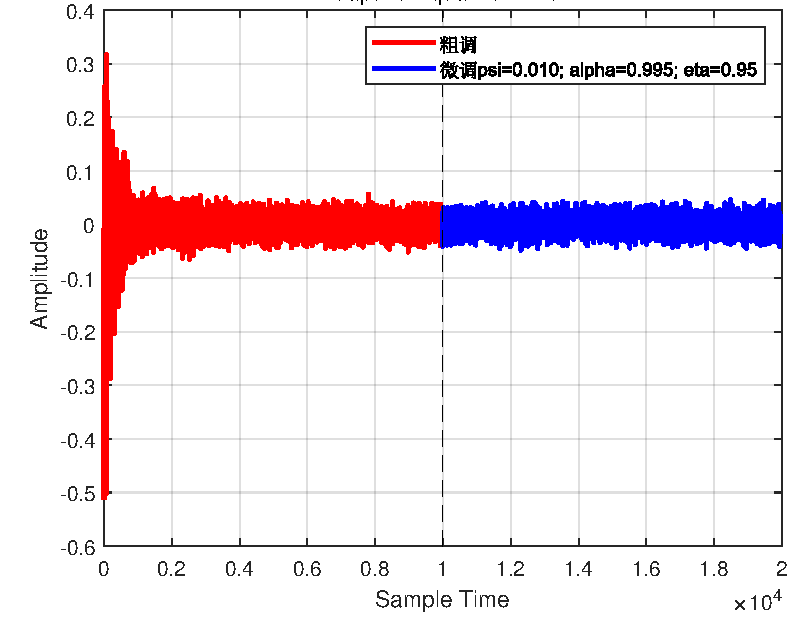
\includegraphics[width=.6\textwidth]{float/ch.cnn2/Errors12t12N25rk=5.pdf}
	\caption{数字均衡器误差迭代曲线}
	\label{figure.cnn2.errors}
\end{figure}

完成系数训练后，通过在核心系数前后补零的方式，将每个通道的滤波器长度从25抽头扩展至39抽头（即 $25+14$）。此扩展操作旨在增强滤波器响应的平滑性，为后续自适应均衡器提供更优的收敛引导。表\ref{table:shilie}是对均衡器系数的示意表，数字标识每个系数在数字均衡器中的位置。图\ref{fig:A1}至图\ref{fig:F}为各个分区的均衡器系数值与幅频响应曲线。各通道的响应特性均针对其对应的分区信道特征进行了适配。


\begin{table}[h]
	\centering
	\caption{示例表格}
	\begin{tabular}{|c|c|c|c|c|}
		\hline
		\multicolumn{5}{|c|}{分区均衡器系数示意表} \\ \hline
		1 & 2 & 3 & 4 & 5 \\
		\hline
		6 & 7 & 8 & 9 & 10 \\
		\hline
		11 & 12 & 13 & 14 & 15 \\
		\hline
		16 & 17 & 18 & 19 & 20 \\
		\hline
		21 & 22 & 23 & 24 & 25 \\
		\hline
	\end{tabular}
	\label{table:shilie}
\end{table}


\begin{figure}[H]
	\centering
	\begin{minipage}[c]{0.45\textwidth} % 设置表格的宽度为文本宽度的一半
		\resizebox{\textwidth}{!}{
			\begin{tabular}{|c|c|c|c|c|}
				\hline
				\multicolumn{5}{|c|}{A1分区均衡器系数} \\ \hline
				-0.0098 & 0.0066 & 0.0006 & 0.0111 & 0.0195 \\ \hline 
				0.0054 & -0.0096 & -0.0144 & -0.0047 & 0.0165 \\ \hline 
				0.0321 & 0.0292 & 0.0285 & 0.0485 & 0.0287 \\ \hline 
				0.0000 & -0.0091 & -0.0036 & 0.0042 & 0.0083 \\ \hline 
				0.0059 & 0.0013 & 0.0098 & 0.0092 & -0.0102 \\ \hline 
		\end{tabular}}
	\end{minipage}%
	\hfill
	\begin{minipage}[c]{0.45\textwidth} % 设置图片的宽度为文本宽度的一半减去一些空间
		\centering
		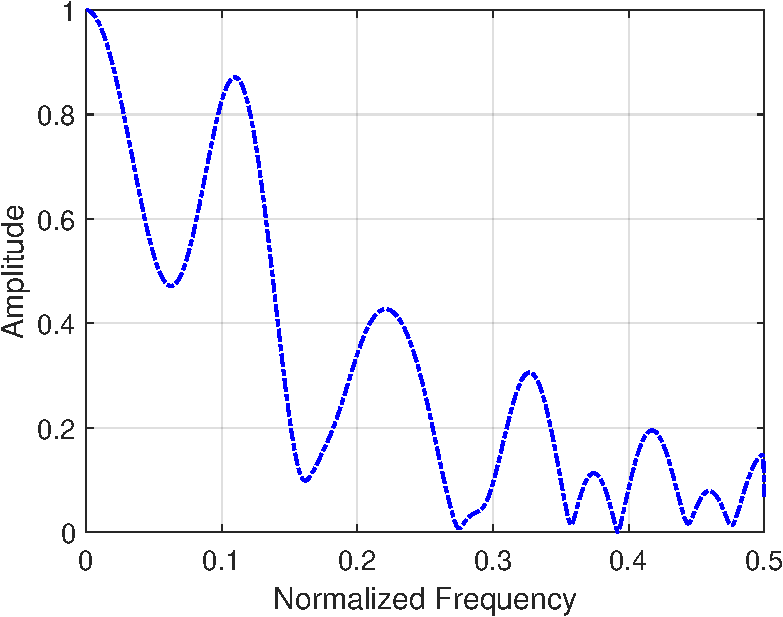
\includegraphics[width=\linewidth]{float/ch.cnn2/InitfirTaps-Ideal-A1.pdf} % 插入图片，替换为你的图片文件名
		% \captionof{figure}{这是图片的标题} % 图片的标题
	\end{minipage}
	\caption{A1分区数字均衡器系数，右侧为响应曲线}
	\label{fig:A1}
\end{figure}

\begin{figure}[H]
	\centering
	\begin{minipage}[c]{0.45\textwidth} % 设置表格的宽度为文本宽度的一半
		\resizebox{\textwidth}{!}{
			\begin{tabular}{|c|c|c|c|c|}
				\hline
				\multicolumn{5}{|c|}{A2分区均衡器系数} \\ \hline
				-0.0115 & 0.0073 & 0.0037 & 0.0162 & 0.0263 \\ \hline 
				0.0126 & -0.0037 & -0.0111 & -0.0038 & 0.0166 \\ \hline 
				0.0327 & 0.0308 & 0.0315 & 0.0532 & 0.0348 \\ \hline 
				0.0064 & -0.0041 & -0.0004 & 0.0059 & 0.0093 \\ \hline 
				0.0064 & 0.0016 & 0.0106 & 0.0107 & -0.0084 \\ \hline 
		\end{tabular}}
	\end{minipage}%
	\hfill
	\begin{minipage}[c]{0.45\textwidth} % 设置图片的宽度为文本宽度的一半减去一些空间
		\centering
		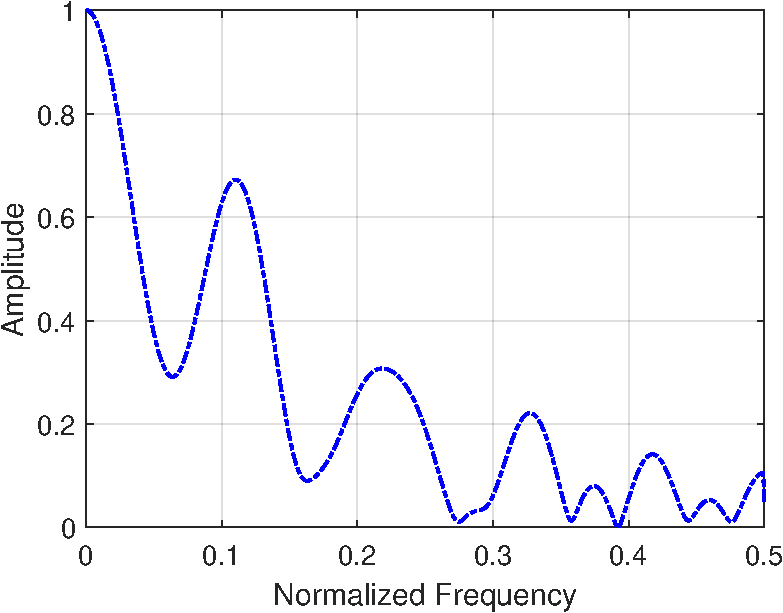
\includegraphics[width=\textwidth]{float/ch.cnn2/InitfirTaps-Ideal-A2.pdf} % 插入图片，替换为你的图片文件名
		% \captionof{figure}{这是图片的标题} % 图片的标题
	\end{minipage}
	\caption{A2分区数字均衡器系数，右侧为响应曲线}
	\label{fig:A2}
\end{figure}


\begin{figure}[H]
	\centering
	\begin{minipage}[c]{0.45\textwidth} % 设置表格的宽度为文本宽度的一半
		\resizebox{\textwidth}{!}{
			\begin{tabular}{|c|c|c|c|c|}
				\hline
				\multicolumn{5}{|c|}{B分区均衡器系数} \\ \hline
				0.0030 & 0.0093 & -0.0113 & -0.0107 & -0.0002 \\ \hline 
				-0.0022 & -0.0016 & 0.0060 & 0.0215 & 0.0405 \\ \hline 
				0.0493 & 0.0404 & 0.0390 & 0.0644 & 0.0538 \\ \hline 
				0.0312 & 0.0198 & 0.0142 & 0.0054 & -0.0064 \\ \hline 
				-0.0174 & -0.0201 & -0.0016 & 0.0092 & -0.0034 \\ \hline 
		\end{tabular}}
	\end{minipage}%
	\hfill
	\begin{minipage}[c]{0.45\textwidth} % 设置图片的宽度为文本宽度的一半减去一些空间
		\centering
		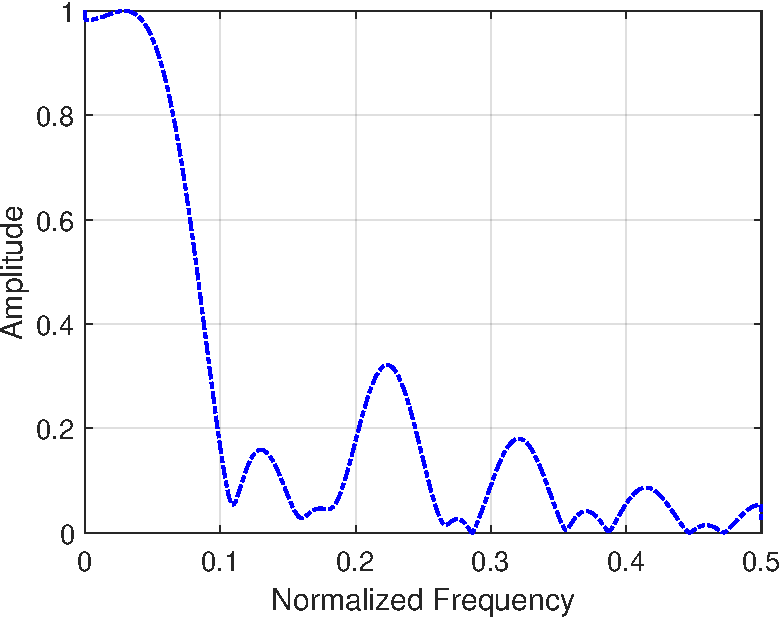
\includegraphics[width=\textwidth]{float/ch.cnn2/InitfirTaps-Ideal-B.pdf} % 插入图片，替换为你的图片文件名
		% \captionof{figure}{这是图片的标题} % 图片的标题
	\end{minipage}
	\caption{B分区数字均衡器系数，右侧为响应曲线}
	\label{fig:B}
\end{figure}

\begin{figure}[H]
	\centering
	\begin{minipage}[c]{0.45\textwidth} % 设置表格的宽度为文本宽度的一半
		\resizebox{\textwidth}{!}{
			\begin{tabular}{|c|c|c|c|c|}
				\hline
				\multicolumn{5}{|c|}{D分区均衡器系数} \\ \hline
				0.0055 & 0.0077 & -0.0142 & -0.0128 & -0.0008 \\ \hline 
				-0.0015 & -0.0004 & 0.0067 & 0.0211 & 0.0392 \\ \hline 
				0.0479 & 0.0404 & 0.0405 & 0.0669 & 0.0569 \\ \hline 
				0.0338 & 0.0209 & 0.0136 & 0.0042 & -0.0072 \\ \hline 
				-0.0171 & -0.0187 & -0.0005 & 0.0080 & -0.0081 \\ \hline
		\end{tabular}}
	\end{minipage}%
	\hfill
	\begin{minipage}[c]{0.45\textwidth} % 设置图片的宽度为文本宽度的一半减去一些空间
		\centering
		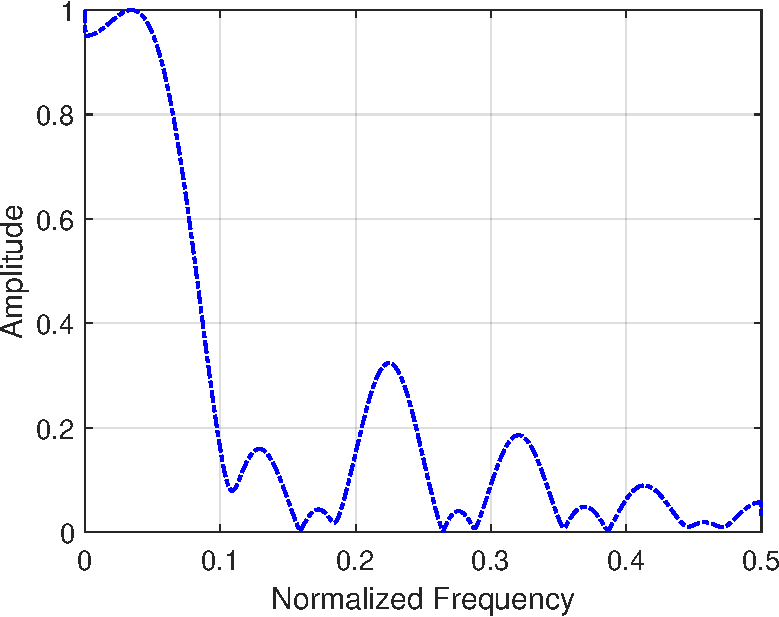
\includegraphics[width=\textwidth]{float/ch.cnn2/InitfirTaps-Ideal-D.pdf} % 插入图片，替换为你的图片文件名
		% \captionof{figure}{这是图片的标题} % 图片的标题
	\end{minipage}
	\caption{D分区数字均衡器系数，右侧为响应曲线}
	\label{fig:D}
\end{figure}

\begin{figure}[H]
	\centering
	\begin{minipage}[c]{0.45\textwidth} % 设置表格的宽度为文本宽度的一半
		\resizebox{\textwidth}{!}{
			\begin{tabular}{|c|c|c|c|c|}
				\hline
				\multicolumn{5}{|c|}{E分区均衡器系数} \\ \hline
				0.0100 & -0.0198 & -0.0061 & -0.0129 & -0.0192 \\ \hline 
				-0.0018 & -0.0009 & -0.0215 & -0.0423 & -0.0454 \\ \hline 
				-0.0187 & 0.0192 & 0.0200 & 0.0294 & 0.0537 \\ \hline 
				0.0304 & 0.0018 & -0.0135 & -0.0160 & -0.0120 \\ \hline 
				-0.0140 & -0.0163 & -0.0038 & 0.0067 & 0.0066 \\ \hline 
		\end{tabular}}
	\end{minipage}%
	\hfill
	\begin{minipage}[c]{0.45\textwidth} % 设置图片的宽度为文本宽度的一半减去一些空间
		\centering
		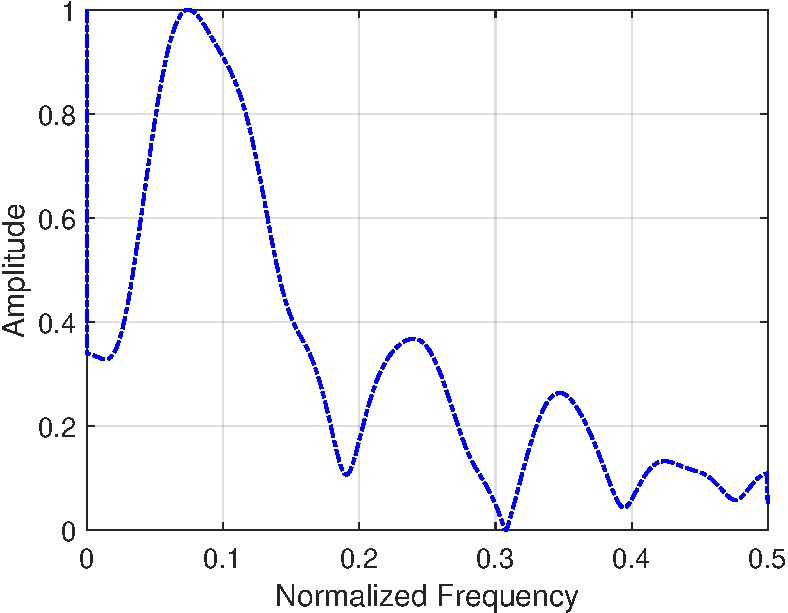
\includegraphics[width=\textwidth]{float/ch.cnn2/InitfirTaps-Ideal-E.pdf} % 插入图片，替换为你的图片文件名
		% \captionof{figure}{这是图片的标题} % 图片的标题
	\end{minipage}
	\caption{E分区数字均衡器系数，右侧为响应曲线}
	\label{fig:E}
\end{figure}

\begin{figure}[H]
	\centering
	\begin{minipage}[c]{0.45\textwidth} % 设置表格的宽度为文本宽度的一半
		\resizebox{\textwidth}{!}{
			\begin{tabular}{|c|c|c|c|c|}
				\hline
				\multicolumn{5}{|c|}{F分区均衡器系数} \\ \hline
				0.0120 & 0.0005 & -0.0144 & -0.0109 & -0.0037 \\ \hline 
				-0.0113 & -0.0160 & -0.0072 & 0.0092 & 0.0262 \\ \hline 
				0.0326 & 0.0308 & 0.0437 & 0.0084 & -0.0412 \\ \hline 
				-0.0390 & -0.0217 & -0.0061 & 0.0016 & -0.0010 \\ \hline 
				-0.0004 & 0.0015 & -0.0172 & -0.0153 & 0.0209 \\ \hline 
		\end{tabular}}
	\end{minipage}%
	\hfill
	\begin{minipage}[c]{0.45\textwidth} % 设置图片的宽度为文本宽度的一半减去一些空间
		\centering
		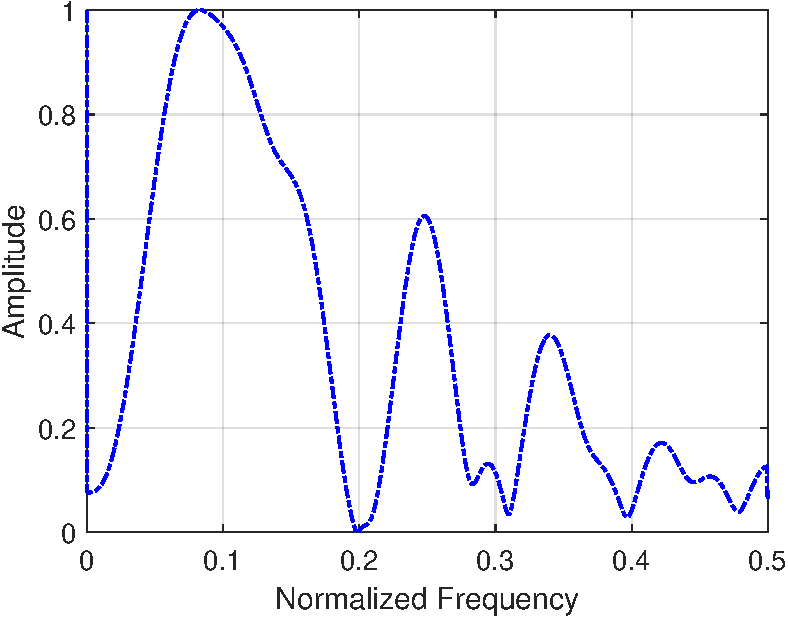
\includegraphics[width=\textwidth]{float/ch.cnn2/InitfirTaps-Ideal-F.pdf} % 插入图片，替换为你的图片文件名
		% \captionof{figure}{这是图片的标题} % 图片的标题
	\end{minipage}
	\caption{F分区数字均衡器系数，右侧为响应曲线}
	\label{fig:F}
\end{figure}

为进一步验证数字均衡器的预处理效果，对均衡前后的信号分布进行了对比分析。图\ref{fig:rk}展示了原始有噪声回读信号的分布直方图，其分布较为离散且不同峰值区间存在明显重叠，表明信号受到严重干扰，各类符号的区分度较低。图\ref{fig:dk}展示了由原始写入数据与预设PR目标卷积生成的理想信号分布，这是维特比检测器进行最优判决的理想参考。图\ref{fig:yk}则展示了经过数字均衡器初步处理后的信号分布。对比图\ref{fig:rk}与图\ref{fig:yk}可以清晰看到，均衡后的信号分布呈现出更高的离散度，不同符号对应的峰值区间分离更为明显，且整体分布形态与理想信号分布（图\ref{fig:dk}）更为接近。这一变化意味着数字均衡器有效地抑制了信道引入的部分线性失真，提升了信号的信噪比与可区分性，为后续的检测环节创造了有利条件。

\begin{figure}[h]
	\centering
	\begin{minipage}[b]{0.3\textwidth}
		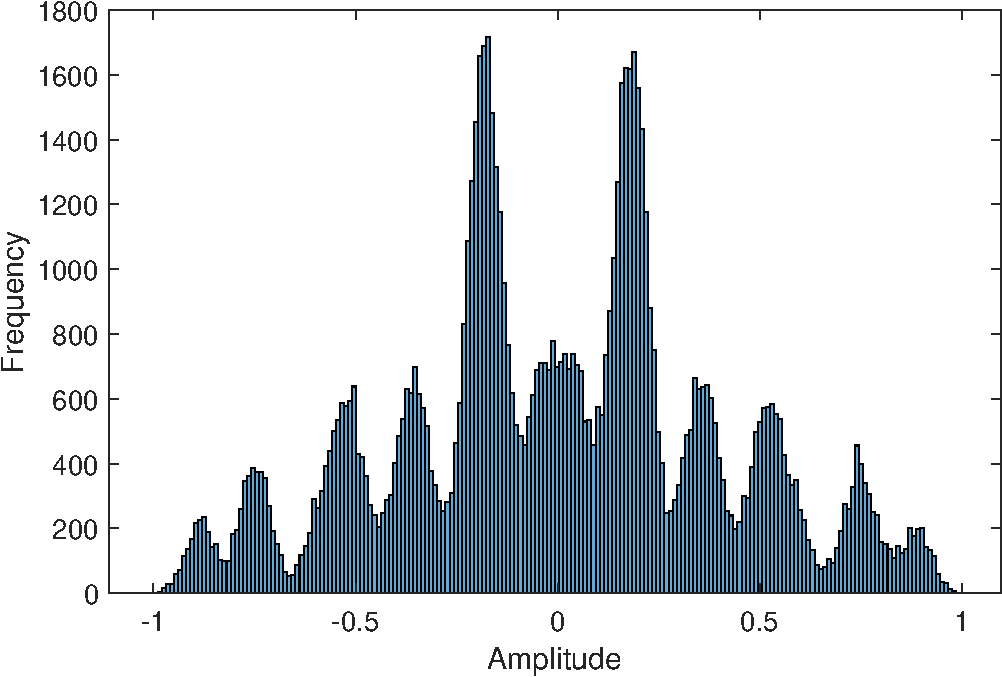
\includegraphics[width=\textwidth]{float/ch.cnn2/rkallHistogram.pdf}
		\caption{回读信号分布图}
		\label{fig:rk}
	\end{minipage}
	\hfill % 用于在两个子图之间添加一些水平空间
	\begin{minipage}[b]{0.3\textwidth}
		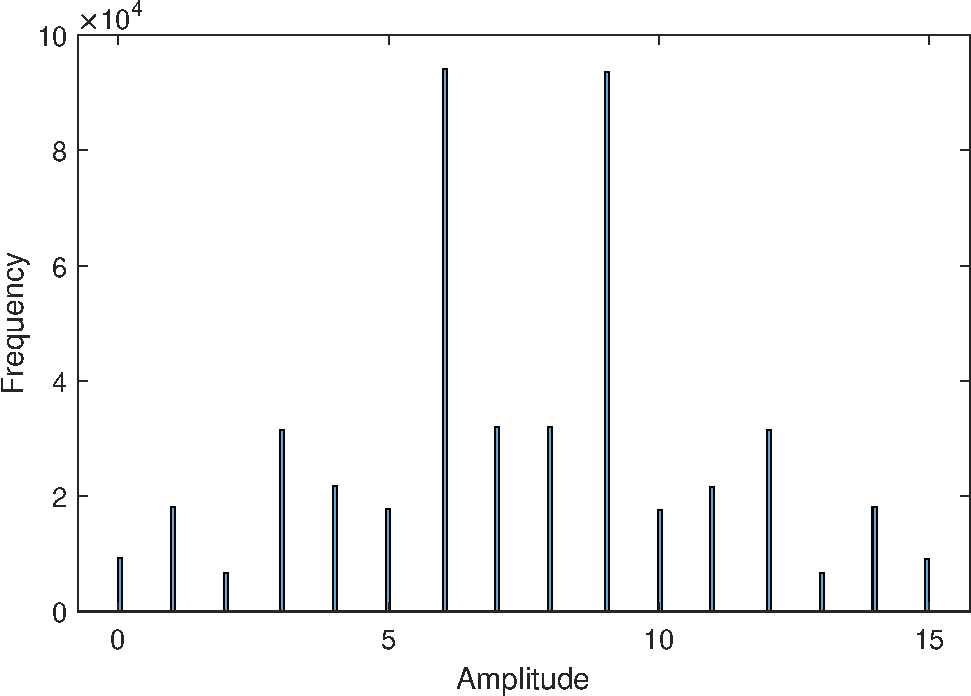
\includegraphics[width=\textwidth]{float/ch.cnn2/dkHistogramGpr7-4.pdf}
		\caption{理想信号分布图}
		\label{fig:dk}
	\end{minipage}
	\hfill % 用于在两个子图之间添加一些水平空间
	\begin{minipage}[b]{0.3\textwidth}
		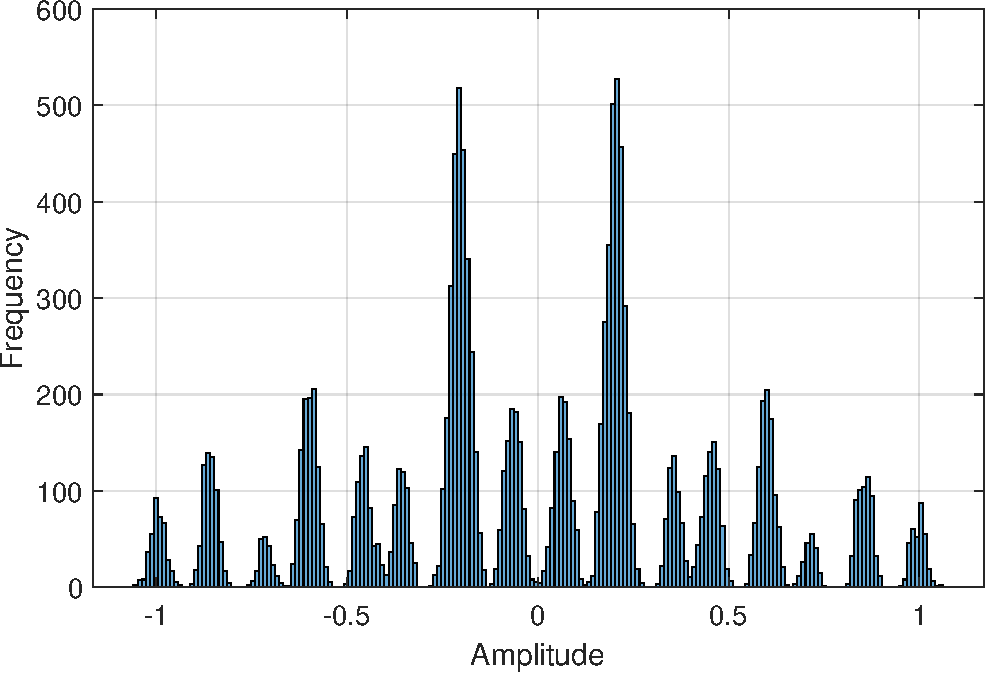
\includegraphics[width=\textwidth]{float/ch.cnn2/yk-rk5t5N13.pdf}
		\caption{均衡后信号分布图}
		\label{fig:yk}
	\end{minipage}
\end{figure}

\textbf{自适应均衡与整体系统性能验证}

在数字均衡器提供良好初始条件的基础上，对包含复杂复合噪声的8万比特数据样本进行了完整的自适应均衡与检测流程测试。自适应均衡器采用符号-误差LMS算法进行在线系数更新，学习速率设置为 $\mu = 4.0376 \times 10^{-4}$。为模拟实际系统中数据分段处理的情况，实验将8万比特数据分为8个连续的段落（每段1万比特），并在处理完每个段落后更新一次均衡器系数。

图\ref{fig:errorsN39}展示了整个处理过程中均衡误差的迭代曲线。从曲线中可以观察到两个关键现象：首先，在处理第一个数据段落（首轮）时，均衡误差相对较大，这符合系统从初始状态开始自适应收敛的预期。其次，在后续的每一轮处理开始时，误差曲线均会出现一个较小范围的瞬时抖动，随后迅速收敛并稳定在较低水平。这一抖动源于每轮开始时，系数更新所依赖的检测结果（用于生成参考信号 $d_k$）本身存在一定误差。随着均衡器系数不断根据新的误差信息进行微调，系统能够快速适应并跟踪信道特征，使得误差在每轮内迅速下降并保持稳定。图\ref{fig:fir}展示了经过8轮自适应更新后最终得到的自适应均衡器系数，这些系数是系统针对当前噪声与干扰环境优化后的结果。

\begin{figure}[h]
	\centering
	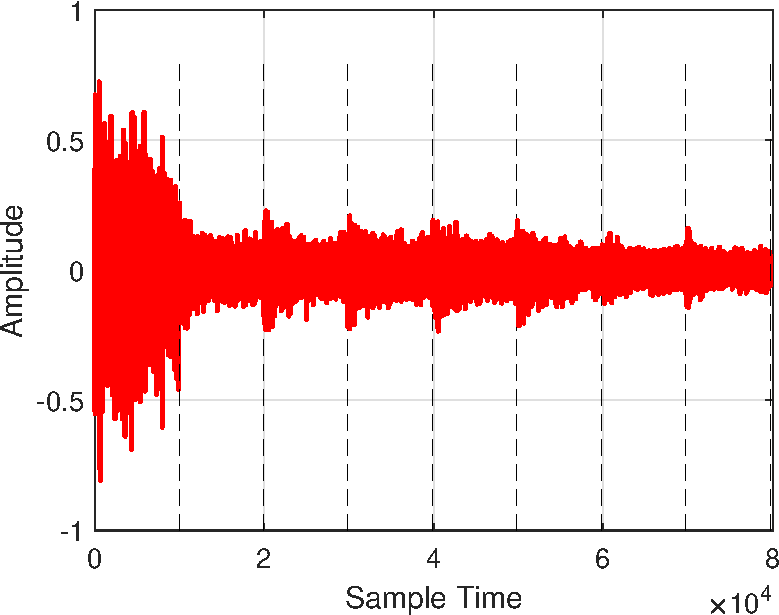
\includegraphics[width=\textwidth]{float/ch.cnn2/errorsN39mu0.5vsn.pdf}
	\caption{均衡误差迭代曲线}
	\label{fig:errorsN39}
\end{figure}

\begin{figure}[H]
	\centering
	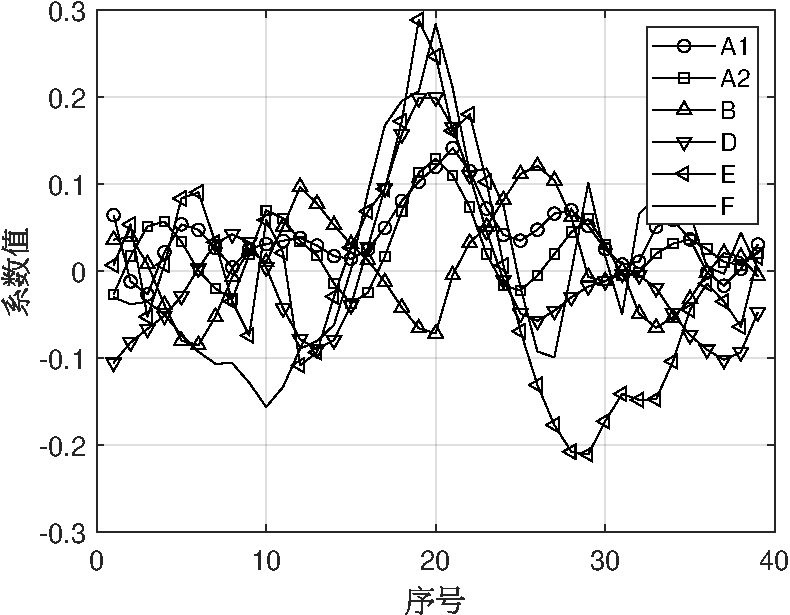
\includegraphics[width=\textwidth]{float/ch.cnn2/firtaps.pdf}
	\caption{均衡器系数}
	\label{fig:fir}
\end{figure}

\textcolor{red}{这下面要改，需要换成单通道时候的结果与多通道结果的对比}

最终，将经过多通道自适应均衡处理后的信号送入集成了状态剪枝与路径存储优化的维特比检测器，并进行d-MLSE信号质量评估。检测器输出的路径度量差分布如图4.19所示。路径度量差直接反映了检测时刻最大似然路径与次优路径之间的“确信度”差异，其分布形态是评估潜在误码风险的关键依据。根据此分布计算得到的d-MLSE指标值为0.1769。与此同时，通过对检测器输出的比特序列与原始写入序列进行比对，得到系统的原始误码率为0.0757。

实验结果表明，本文提出的多通道自适应均衡系统能够有效处理高密度AD光盘在复杂噪声环境下的回读信号。从信号分布变化来看，数字均衡器成功完成了初步的线性补偿与干扰抑制。从误差收敛过程来看，自适应均衡器能够在存在检测误差反馈的情况下实现稳定、快速的跟踪与收敛。最终的误码率与d-MLSE指标表明，系统在经过完整的均衡与检测流程后，能够以较高的可靠性恢复原始数据。尽管原始误码率仍有优化空间，但d-MLSE值提供了一个内在的质量基准，为后续进一步优化（如第五章将探讨的动态PR目标搜索）提供了明确的参考方向和量化依据。与传统单通道均衡方案相比，本系统利用多分区信息进行协同处理，在应对由轨道间串扰等引发的多维干扰方面展现出其架构优势。

\section{本章小结}

